
% Autor: Rami Boutassghount
% Website: https://ramiboutas.com/
% Linkedin: https://www.linkedin.com/in/ramiboutas/
% Twitter: https://twitter.com/ramiboutas
% Telegram: https://t.me/ramiboutas
\documentclass[tikz, convert={density=300}]{standalone}
\usepackage{pgfplots}
\tikzstyle{load}=[ultra thick,-latex]
\tikzstyle{stress}=[-latex]
\tikzstyle{dim}=[latex-latex]
\tikzstyle{axis}=[-latex,black!55]

\begin{document}
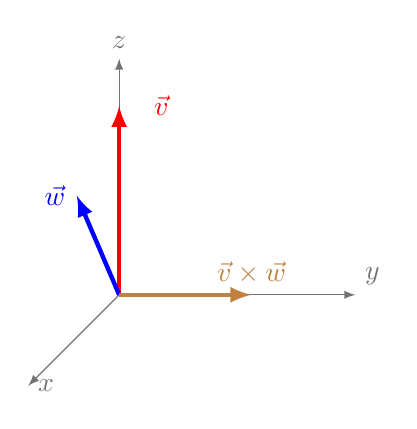
\begin{tikzpicture}[cm={-1,-1,1,0,(0,0)},x=3.85mm,z=-1cm,scale=2]
	
	\coordinate (O) at (0,0,0);
	\draw[axis] (O) -- ++(1.5,0,0) node[right] {$x$};
	\draw[axis] (O) -- ++(0,1.5,0) node[above right] {$y$};
	\draw[axis] (O) -- ++(0,0,1.5) node[above] {$z$};	
	
	\def\xO{0}
	\def\yO{0}
	\def\zO{0}
	
	\def\vx{0}
	\def\vy{0}
	\def\vz{1.2}
	
	\def\wx{0.7}
	\def\wy{0}
	\def\wz{0.9}
		
	\draw[load, red] (\xO,\yO,\zO) -- ++(\vx,\vy,\vz) node[right,xshift=0.3cm] {$\vec{v}$};	
	\draw[load, blue] (\xO,\yO,\zO) -- ++(\wx,\wy,\wz) node[left,xshift=0cm] {$\vec{w}$};	
	\draw[load, brown] (\xO,\yO,\zO) -- ++(\vy*\wz-\vz*\wy, \vz*\wx-\vx*\wz, \vx*\wy-\wx*\vy) node[above,xshift=0cm] {$\vec{v} \times \vec{w}$};	

	\end{tikzpicture} %
\end{document}
